% Le partitionnement de données : découvrir des motifs dans un corpus

\subsection{Regrouper les images : principes et jeux de données}
    \subsubsection{L'apprentissage non-supervisé}
    Le \textit{clustering} est une tâche d'apprentissage non-supervisé : contrairement aux tâches décrites dans les chapitres précédents, elle ne fait pas l'objet d'un entraînement à partir de données annotées\footnote{L'un des avantages souvent relevés pour l'apprentissage non-supervisé est l'absence de nécessité de l'intervention en amont de la création du modèle d'un chercheur ayant une expertise sur les données traitées, car il n'existe pas d'étape de création d'un jeu de données d'entraînement annoté.}, et fait appel à d'autres critères qu'une vérité de terrain pour son évaluation\footcite{Clustering}. L'étape de validation est ainsi basée sur un jeu de données dont les critères sont plus flous que pour les tâches précédemment mentionnées, et peuvent consister, par exemple, à considérer que des sources spécifiques se doivent d'être proches dans l'espace pour que le modèle soit jugé performant. La différence fondamentale entre apprentissage supervisé et non-supervisé réside dans les attentes qui entourent les résultats du modèle développé. Dans le cas d'un apprentissage supervisé, la volonté est d'obtenir un modèle apte à la généralisation, qui peut produire des prédictions pertinentes sur de nouvelles données. Les enjeux de l'apprentissage non-supervisé sont différents : il est attendu du modèle d'apporter un regard sur un ensemble de données, et d'y discerner des motifs que le chercheur ne peut anticiper\footcite{deluaSupervisedVsUnsupervised2021}. Ainsi, l'apprentissage non-supervisé est idéal pour une tâche telle que le partitionnement de données, pour laquelle il est complexe de construire des vérités de terrains, ou d'annoter des jeux de données d'entraînement volumineux. L'intérêt d'un algorithme de \textit{clustering} réside dans le regard nouveau qu'il peut apporter sur un ensemble de données, en discernant des motifs qu'un observateur humain ne peut observer.
    
    \subsubsection{Données d'entrée et extraction des caractéristiques}
    L'application à un corpus complet -- tels que les divers corpus mentionnés dans ce mémoire, qui comptent des centaines de milliers d'images -- d'un algorithme de \textit{clustering} implique le traitement d'un volume massif de données non-classifiées et non-annotées, qui nécessite alors une puissance de calcul importante pour chacune des étapes nécessaires à ce processus. L'entraînement d'un modèle de \textit{clustering} non-supervisé requiert une quantité massive de données\footnote{Le volume des jeux de données d'entraînement est plus important que pour l'apprentissage supervisé, notamment.} pour produire des résultats pertinents : les réseaux de neurones et modèles de partitionnement de données utilisés dans les exemples mentionnés à la suite de ce chapitre sont, le plus souvent, des modèles pré-entraînés que les projets ajustent à leurs besoins\footcite{castellanoDeepLearningApproach2022}.
    
    Le \textit{clustering} s'appuyant sur des points dans un espace de grande dimension, il est nécessaire pour un projet souhaitant employer un tel algorithme d'établir les critères selon lesquels les données sont placées dans l'espace. Ces critères ne sont pas déterminés manuellement, mais sont calculés à partir de caractéristiques, ou \textit{features}, extraites des données sources par un \cnn. La méthode \acrfull{delius}\footcite{castellanoDeepLearningApproach2022}, développée par Giovanna Castellano et Gennaro Vessio, propose une \textit{pipeline} pour la création de \textit{clusters} à partir d'un corpus d'œuvres d'art provenant d'époques et de mouvements divers. La chaîne de traitement proposée inclut une extraction de caractéristiques par un réseau DenseNet121\footnote{DenseNet121 est un réseau neuronal à convolution : les caractéristiques extraites en prévision du partitionnement de données correspondent aux caractéristiques identifiées par le réseau, selon les techniques explicitées dans la partie \ref{neuralNets}.} ; ces \textit{features} sont ensuite fournies au modèle de \textit{clustering} pour le traitement des données et leur regroupement en fonction de ces caractéristiques, puis projetées dans un espace en deux dimensions pour en faciliter la visualisation. Cependant, si cette \textit{pipeline} automatique a fait ses preuves, et a permis au projet des résultats satisfaisants en termes de regroupement des œuvres d'art, son intégration à une application en ligne, mise à disposition des chercheurs, soulève des questions supplémentaires. 
    
    En effet, l'extraction des caractéristiques est effectuée à partir d'un jeu de données déterminé, à un instant précis, pour fournir les paramètres de l'algorithme de \textit{clustering}, qui performe ensuite sur ce même jeu de données. Dans le cas d'une application mise à disposition du public, telle que l'application prévue par le projet \eida\footnote{Parmi les fonctionnalités prévues par \eida, le partitionnement de données compte parmi les outils d'analyse des sources et de traitement pour l'édition des diagrammes astronomiques.}, le jeu de données sur lequel performer les regroupements ne peut être considéré comme une instance fixe, et l'utilisation de l'application par les chercheurs implique une expansion constante de ce jeu de données. Pour maintenir les performances du modèle de partitionnement, il faut ainsi considérer la nécessité éventuelle d'un re-calcul fréquent des caractéristiques, pour conserver un modèle adapté aux sources qu'il regroupe. Au contraire, il est envisageable de conserver les caractéristiques extraites, en considérant le jeu de données initial comme suffisamment représentatif des sources qui seront traitées par l'application à la demande des chercheurs. Les méthodes actuelles de regroupement des données par vision artificielle posent ainsi la question de la pérennité des outils développés face à la possible diminution des performances du modèle en cas d'enrichissement du jeu de données de base, et de leur pertinence sur la durée. Ces questionnements revêtent une importance particulières dans le contexte de développement d'un outil dédié aux traitement des sources, ayant pour vocation de proposer des rapprochements qui ouvrent des pistes pertinentes -- ou intéressantes -- dans le cadre de recherches historiques.
    
\subsection{Le partitionnement de données pour les sources visuelles}
    \subsubsection{Pré-sélection, correction et intervention du chercheur}
    En tant que tâche d'apprentissage non-supervisée, le \textit{clustering} ne nécessite pas de production d'un jeu de données annoté pour l'entraînement du modèle. Il existe cependant un ensemble d'interventions nécessaires du chercheur, au fil de la chaîne de traitement, qui permettent de s'assurer de la cohérence et de la pertinence des résultats obtenus.
    
    Pour assurer une meilleure performance du modèle, des résultats plus satisfaisants et un temps de calcul réduit, il est préférable de procéder, en amont du partitionnement, à la sélection d'un ensemble restreint de sources à traiter parmi les données globales du projet. Du point de vue du développement d'une application à destination des chercheurs, il est possible d'envisager la mise à disposition d'une interface pour la sélection des images sur lesquelles effectuer le \textit{clustering}. Le projet \eida envisage ainsi une interface qui permettrait aux chercheurs de créer des sous-corpus à partir des diagrammes vectorisés, navigables par le biais de leurs métadonnées, pour appliquer à un ensemble d'intérêt un algorithme de regroupement qui pourrait proposer des liens insoupçonnés entre les données, et trouver des similarités entre des diagrammes à partir de caractéristiques définies pour le modèle en amont de ce développement.
    
    Le partitionnement de données n'étant pas basé sur des attentes spécifiques aux pratiques définies, il n'est pas envisageable de proposer une correction des annotations comme effectuée sur les résultats d'algorithmes de détection d'objet ou de vectorisation. Une intervention humaine\footcite{deluaSupervisedVsUnsupervised2021} à l'issue de la chaîne de traitement est cependant nécessaire, pour s'assurer de la validité des résultats produits par l'algorithme de \textit{clustering} : un regard porté sur les prédictions par un chercheur, fort d'une expertise sur les sources étudiées, permet de s'assurer de la pertinence du modèle utilisé et de la cohérence des résultats publiés.
    
    \subsubsection{Le \textit{clustering}, porteur de découvertes en histoire de l'art ?}
    \begin{figure}[h]
    	\centering
    	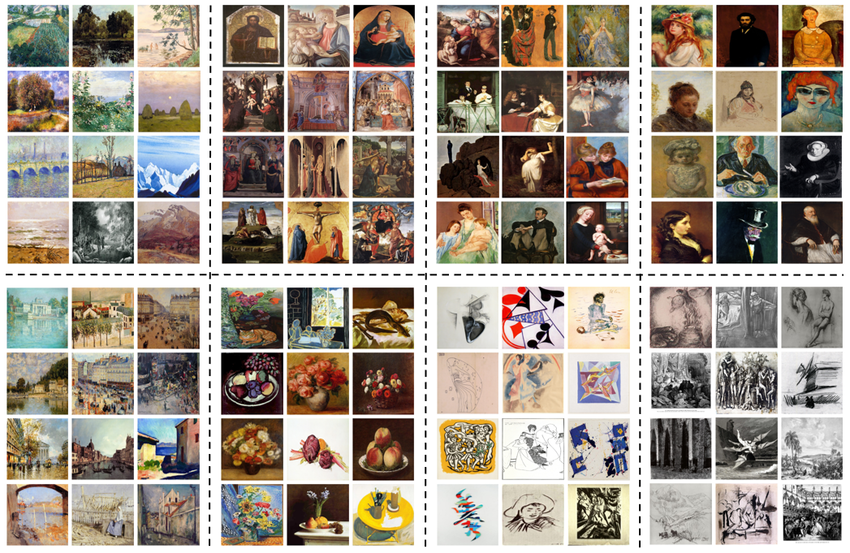
\includegraphics[width=15cm]{images/delius_global_clusters.png}
    	\caption{Groupes prédits par la méthode \acrshort{delius} dans l'ensemble du jeu de données}
    	\label{fig:delius_global_clusters}
    \end{figure}

	À titre d'exemple, les résultats de l'application de la méthode \acrshort{delius} à un jeu de données global\footnote{Le jeu de données utilisé est récupéré de WikiArt, et compte 78 978 tableaux, dessins et illustrations provenant de périodes variées, sans restriction de thème et de genre. \cite{ArtGANWikiArt}} témoignent d'une répartition basée essentiellement sur le sujet des œuvres d'art traitées (fig. \ref{fig:delius_global_clusters}). Ainsi, les \textit{clusters} formés regroupent les portraits, les paysages, les natures mortes, et ne semble pas effectuer de distinction de style ou de mouvement : les résultats, dont la précision ne dépasse jamais 50\% d'après les diverses évaluations effectuées\footcite{castellanoDeepLearningApproach2022}, \og suggèrent que le modèle tend à regarder le contenu plutôt que les caractéristiques stylistiques pour grouper les tableaux [Traduction personnelle]\footnote{\textit{\og These results suggest that the model tends to look at content rather than stylistic features to group paintings. \fg} \cite{castellanoDeepLearningApproach2022}} \fg.
	
	\begin{figure}[h]
		\centering
		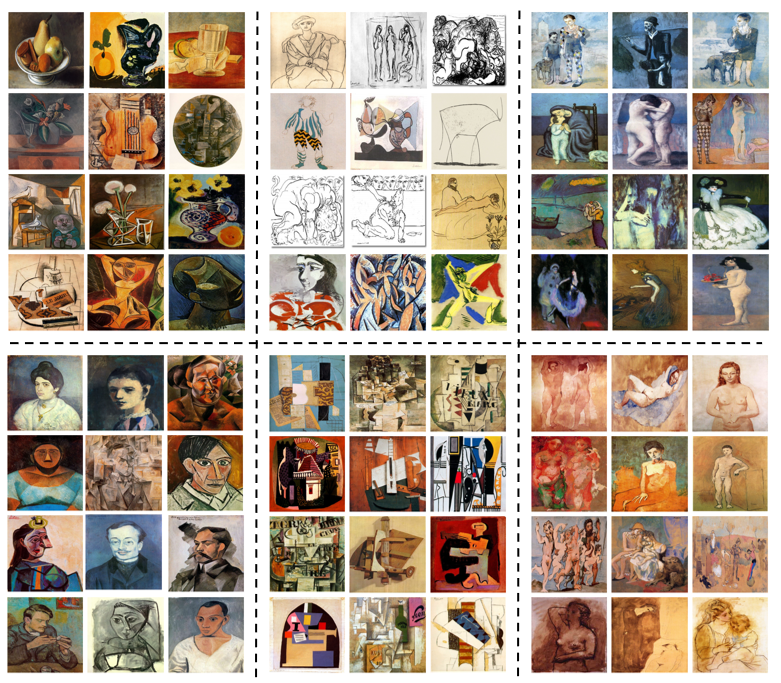
\includegraphics[width=15cm]{images/delius_picasso_clusters.png}
		\caption{Groupes prédits par la méthode \acrshort{delius} dans les œuvres de Picasso}
		\label{fig:delius_picasso_clusters}
	\end{figure}

	La même méthode, appliquée à un sous-corpus restreint composé de 762 œuvres de Pablo Picasso, présente des résultats plus proches des attentes qui entourent le partitionnement de données pour l'analyse de sources en histoire de l'art. Parmi les six groupes constitués (fig. \ref{fig:delius_picasso_clusters}), nous observons quatre groupes dont les œuvres témoignent de sujets similaires, indépendamment du style. Le point d'intérêt se situe cependant dans deux groupes formés majoritairement d'œuvres liées aux périodes bleues et roses de Picasso, dont les similarités vont au-delà du contenu des tableaux, et semblent prendre en compte des aspects liés au style et à la couleur \footcite{castellanoDeepLearningApproach2022}. Il est cependant nécessaire de tempérer ces conclusions par le constat que, dans l'œuvre de l'artiste choisi, les différences de style et de couleur entre les périodes sont particulièrement marquées, et que ces spécificités du travail de Picasso soutiennent éventuellement les performances de \acrshort{delius}. Si les résultats de cette méthode restent, à ce jour, peu satisfaisants, il n'en sont pas moins prometteurs en termes d'analyse par la vision artificielle de corpus d'œuvres d'art\footnote{D'autres approches, telles que QArt-Learn, ont témoigné de meilleures performances pour la catégorisation des œuvres d'art en fonction du style. Cependant, la méthode n'ayant été utilisée que sur des oeuvres issues de trois mouvements artistiques, ses capacités de généralisation dans un contexte plus global ne sont pas encore avérées. \cite{falomirCategorizingPaintingsArt2018}}.